\chapter{Cadre général du projet}
\begingroup
\etocsettocstyle{\rule{\linewidth}{\tocrulewidth}\vskip0.5\baselineskip}{\rule{\linewidth}{\tocrulewidth}}
\localtableofcontents 
\endgroup
\newpage

\section{Introduction}
Ce chapitre est consacré à la présentation du cadre général de notre projet.  
Dans un premier temps, nous présentons la société d’accueil. Par la suite, nous exposons le contexte du projet, afin de comprendre la problématique à laquelle nous avons souhaité répondre. Ensuite, nous détaillons la méthodologie que nous avons adoptée pour le développement de notre projet. Nous terminons par la présentation des solutions existantes sur le marché, accompagnée d’une étude comparative de celles-ci, ainsi que de la solution que nous avons proposée.

\section{Société d’accueil}
Notre stage a été effectué au sein de la société Mobelite~\cite{mobelite}, située à Monastir. Il s’agit d’une filiale offshore de la société Mobelite France. Elle est spécialisée dans le conseil en stratégie mobile, la conception et le développement d’applications mobiles et de sites web, ainsi que dans le marketing mobile. Elle dispose d’équipes commerciales et marketing à Paris (France), et d’équipes de développement à Monastir (Tunisie).
Mobelite possède 12 ans d’expérience et compte une centaine de collaborateurs. Elle a plus de 90 clients, principalement en France, et a réalisé plus de 150 projets. La figure présente le logo de Mobelite.

\begin{figure}[H]
    \centering
    
\includegraphics[scale=0.6]{Figures/mobeliteLogo.png}
    \caption{Logo de Mobelite}
    \label{fig:mobelite_logo}
\end{figure}

\section{Contexte du projet}
MindCare-AI est une solution innovante qui combine l’intelligence artificielle, l’analyse physiologique et la reconnaissance des émotions afin d’offrir un suivi personnalisé de la santé mentale.  
Notre objectif principal est d’améliorer le bien-être des patients en détectant précocement d’éventuelles dégradations de leur état émotionnel ou physiologique, et en leur proposant un accompagnement thérapeutique multimodal.  
Grâce à l’intégration de modèles d’IA, de questionnaires standardisés et de l’analyse des signaux physiologiques par caméra, MindCare-AI permet d’obtenir une représentation globale, précise et contextualisée de l’état de chaque patient.  
Ces données nous permettent d’adapter l’aide apportée, que ce soit par des recommandations sur mesure, un suivi personnalisé ou des interventions renforcées lorsque cela est nécessaire.  
Le système prend également en compte l’évolution de chaque cas afin d’offrir un accompagnement continu et réactif, renforçant l’efficacité des prises en charge et aidant chaque patient à se sentir soutenu, écouté et entouré, sans nécessiter de déplacements ni de consultations physiques.  
Ainsi, MindCare-AI s’affirme comme un outil innovant, accessible, flexible et proche des besoins des patients, pouvant s’intégrer dans leur quotidien de manière non invasive et sécurisée, tout en faisant progresser la médecine prédictive et préventive dans le domaine de la santé mentale.  
Le système intègre également un chatbot thérapeutique, capable d’interagir avec le patient, d’évaluer son état émotionnel à travers le langage naturel et de proposer des conseils adaptés en temps réel.

\section{Problématique}
Les troubles mentaux, tels que la dépression, l’anxiété, le stress chronique ou les troubles de l’humeur, touchent aujourd’hui une part importante de la population mondiale. Selon l’Organisation mondiale de la santé (OMS)~\cite{oms_mental_health}, près d’une personne sur quatre sera affectée par un trouble mental au cours de sa vie. Malgré cette prévalence élevée, la prise en charge de la santé mentale demeure un défi majeur pour les systèmes de santé, pour plusieurs raisons :
\begin{itemize}
    \item \textbf{Difficulté d’accès aux soins spécialisés} : Le nombre de professionnels de santé mentale est insuffisant par rapport à la demande, en particulier dans les zones rurales ou défavorisées. Les délais d’attente pour obtenir un rendez-vous peuvent être très longs, ce qui retarde la prise en charge.
    \item \textbf{Stigmatisation et isolement social} : De nombreux patients hésitent à consulter par peur du jugement ou du rejet social, ce qui aggrave leur isolement et retarde la détection des troubles.
    \item \textbf{Complexité du diagnostic} : Les troubles mentaux présentent souvent des symptômes variés, subjectifs et fluctuants, rendant leur identification difficile sans un suivi régulier et approfondi. Les outils d’évaluation traditionnels reposent principalement sur des entretiens cliniques, qui peuvent manquer d’objectivité ou être influencés par le contexte.
    \item \textbf{Suivi discontinu et manque de personnalisation} : Le suivi des patients est souvent ponctuel, limité aux consultations en présentiel, et ne tient pas toujours compte de l’évolution quotidienne de l’état émotionnel ou physiologique du patient. Cela peut conduire à une détection tardive des rechutes ou à une adaptation insuffisante des interventions thérapeutiques.
    \item \textbf{Barrières technologiques et économiques} : Les solutions existantes nécessitent parfois des équipements coûteux ou une expertise technique, ce qui limite leur accessibilité pour le grand public.
\end{itemize}
Dans ce contexte, il nous a semblé crucial de repenser les approches traditionnelles et de tirer parti des avancées technologiques, notamment de l’intelligence artificielle, pour proposer des outils innovants, accessibles, continus et personnalisés, capables d’accompagner efficacement les patients dans la gestion de leur santé mentale.
\section{Etude d'existance}

\subsection{Analyse des signaux vitaux}

L'analyse des signaux vitaux à distance a connu un développement significatif ces dernières années, particulièrement avec l'essor de la photopléthysmographie à distance (rPPG). Plusieurs solutions commerciales et académiques proposent des approches variées pour cette problématique.Par exemple 

\textbf{Binah.ai} ~\cite{binah_ai}représente l'une des solutions les plus avancées du marché. Cette plateforme utilise l'intelligence artificielle pour extraire les signaux vitaux à partir de caméras standards. Elle propose une API capable de mesurer la fréquence cardiaque, la variabilité cardiaque, la fréquence respiratoire, et même d'estimer la pression artérielle. Cependant, cette solution présente des limitations importantes : son coût élevé (plusieurs milliers d'euros par mois), sa dépendance à une connexion internet stable, et ses restrictions d'utilisation dans des environnements contrôlés.

\begin{figure}[H]
    \centering
    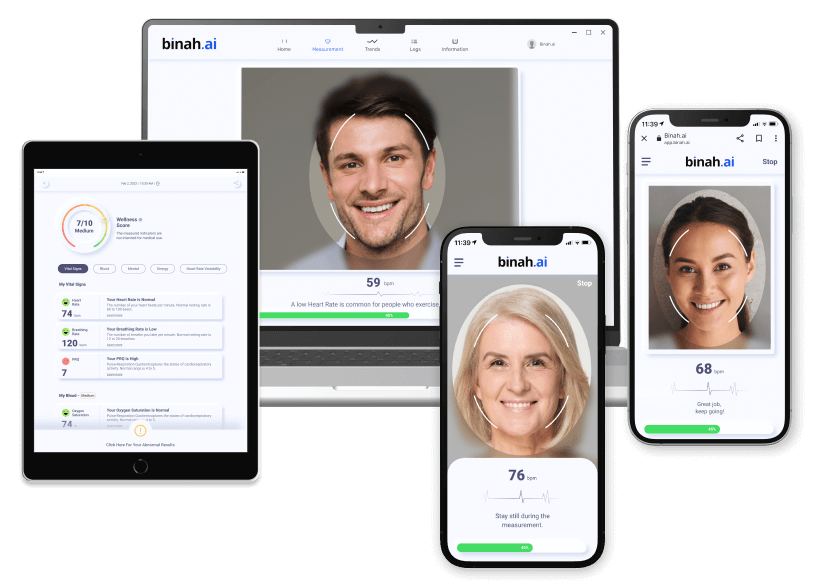
\includegraphics[scale=0.4]{Figures/binah.png}
    \caption{application binah}
    \label{fig:binah_app}
\end{figure}

\textbf{VitalSigns  Philips} constitue une solution hospitalière robuste. Intégrée dans les systèmes de surveillance médicale, elle permet un monitoring continu des patients sans contact. Cette solution excelle dans les environnements cliniques contrôlés mais n'est pas adaptée aux applications grand public en raison de sa complexité et de son coût prohibitif.

\begin{figure}[H]
    \centering
    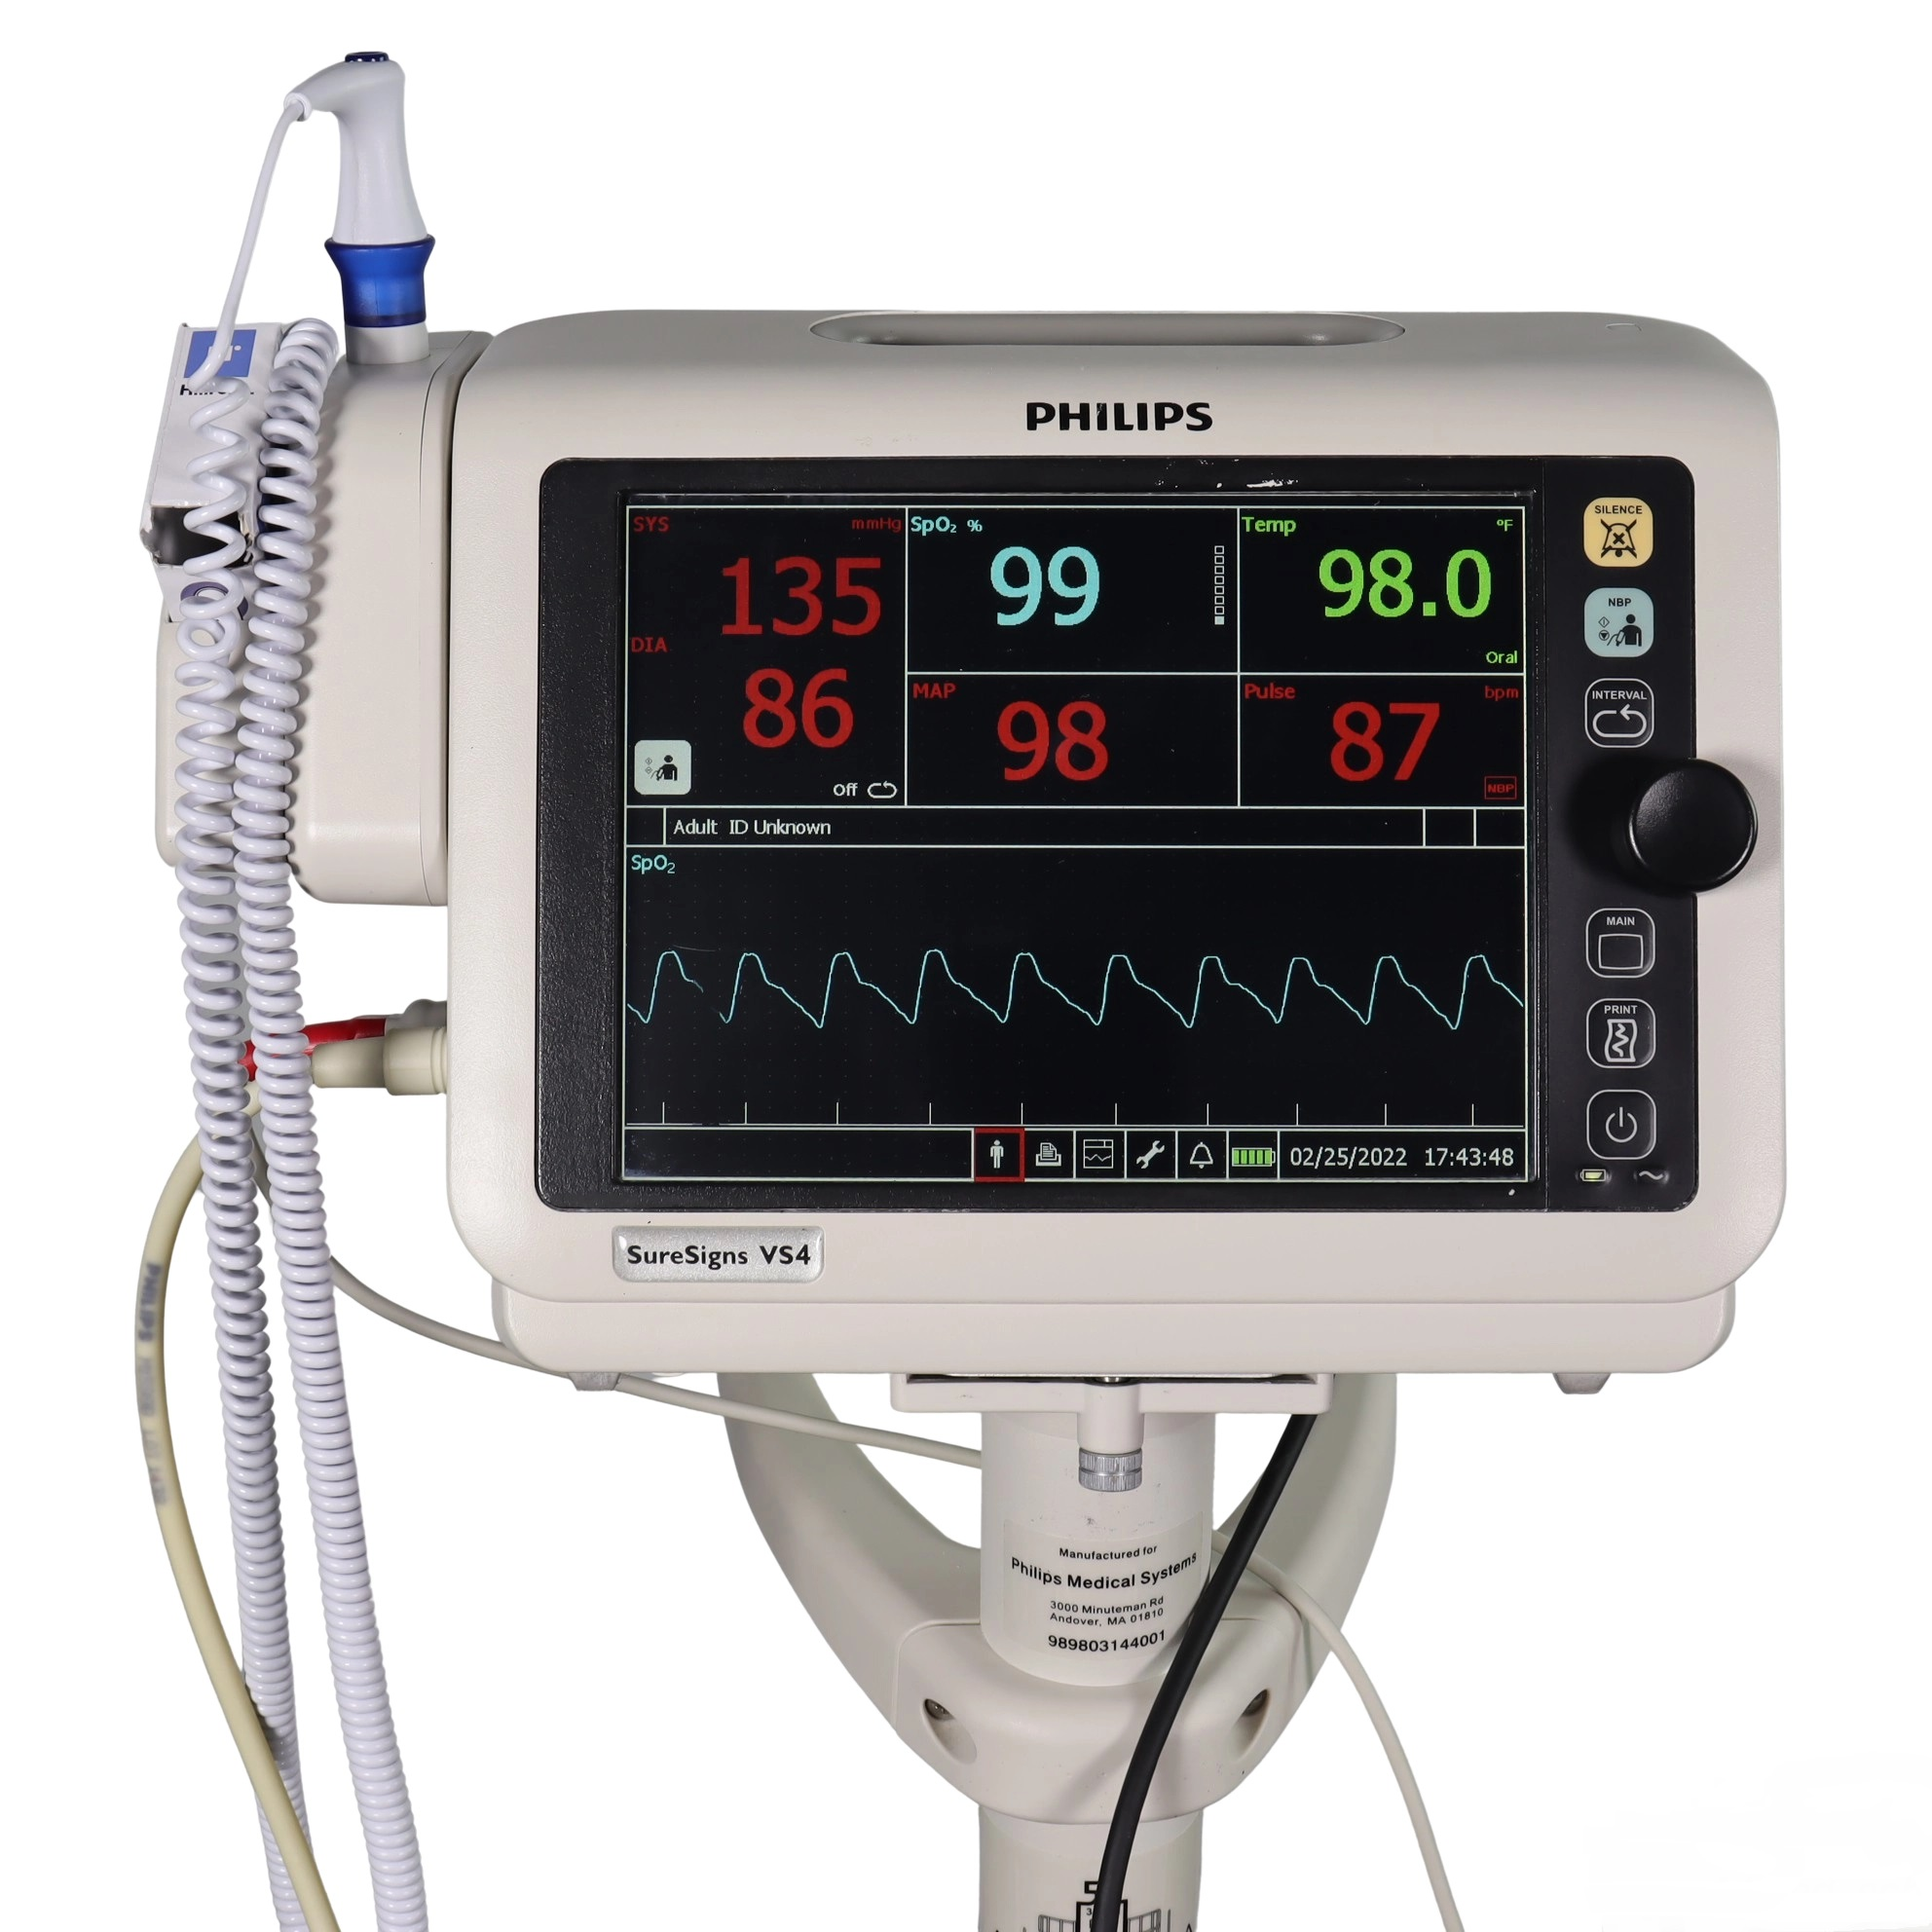
\includegraphics[scale=0.1]{Figures/Philips.png}
    \caption{VitalSigns  Philips}
    \label{fig:philips_vitalsigns}
\end{figure}

\subsubsection*{Tableau comparatif des solutions d'analyse des signaux vitaux}

\begin{table}[h]
\centering
\begin{tabular}{|p{2.2cm}|p{1.8cm}|p{1.8cm}|p{1.8cm}|p{2.8cm}|}
\hline
\textbf{Solution} & \textbf{Type} & \textbf{Coût} & \textbf{Précision} & \textbf{Paramètres mesurés} \\
\hline
Binah.ai & Commercial & Très élevé & Très élevée (< 3\%) & FC, FR, PA \\
\hline
VitalSigns Philips & Hospitalier & Très élevé & Très élevée & FC, FR, SpO2, PA, Température \\
\hline
\textbf{MindCare-AI} & \textbf{Intégré} & \textbf{Gratuit} & \textbf{Très Élevée} & \textbf{FC, PA, état émotionnel} \\
\hline
\end{tabular}
\caption{Comparaison des solutions d'analyse des signaux vitaux}
\label{tab:vitalsigns_comparison}
\end{table}

\textbf{Légende :}
\begin{itemize}
    \item FC : Fréquence Cardiaque 
    \item FR : Fréquence Respiratoire
    \item PA : Pression Artérielle
    \item SpO2 : Saturation en Oxygène
\end{itemize}


\subsection{Chatbots thérapeutiques}

Le domaine des chatbots thérapeutiques et d'accompagnement en santé mentale a connu une croissance exponentielle, particulièrement depuis la pandémie de COVID-19. Ces solutions visent à démocratiser l'accès aux soins psychologiques et à offrir un soutien 24/7 aux personnes en détresse.Par example

\textbf{Woebot} figure parmi les pionniers du secteur. Développé par des psychologues de Stanford, ce chatbot utilise la thérapie cognitivo-comportementale (TCC) pour aider les utilisateurs à gérer leur anxiété et leur dépression. Woebot propose des conversations structurées, des exercices de réflexion et un suivi de l'humeur. Les études cliniques montrent une efficacité significative dans la réduction des symptômes dépressifs. Cependant, Woebot présente des limitations : interactions parfois rigides, manque de personnalisation avancée, et coût d'abonnement mensuel.~\cite{woebot}
\begin{figure}[H]
    \centering
    
\includegraphics[scale=0.4]{Figures/logo.png}
    \caption{Woebot Health}
    \label{fig:woebot_health}
\end{figure}

\textbf{Replika} propose une approche différente en tant que "compagnon IA" personnalisé. Utilisant des modèles de langage avancés, Replika apprend des conversations avec l'utilisateur pour développer une personnalité unique. Bien que non spécifiquement thérapeutique, cette application offre un soutien émotionnel et une écoute active. Ses forces incluent une personnalisation poussée et des conversations naturelles, mais elle manque de fondements thérapeutiques validés scientifiquement.~\cite{replika} 

\begin{figure}[H]
    \centering
    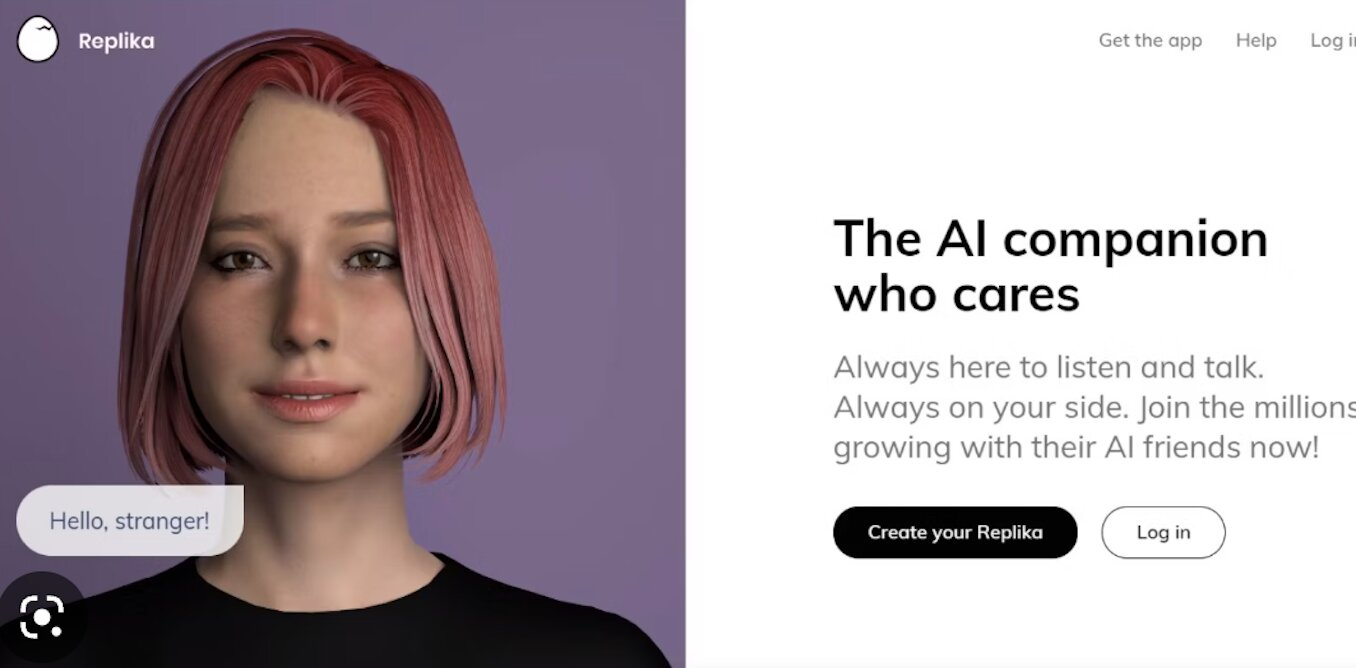
\includegraphics[scale=0.2]{Figures/replika.png}
    \caption{Replika}
    \label{fig:replika_app}
\end{figure}



\subsubsection*{Tableau comparatif des solutions de chatbots }

\begin{table}[H]
\centering
\begin{tabular}{|p{2.5cm}|p{2cm}|p{2.5cm}|p{2.5cm}|}
\hline
\textbf{Solution} & \textbf{Coût} & \textbf{Personnalisé} & \textbf{Intégration} \\
\hline
Woebot & Payant & Moyenne & Limitée \\
\hline
Replika & Payant & Élevée & Faible \\
\hline
\textbf{MindCare-AI} & \textbf{Gratuit} & \textbf{Élevée} & \textbf{Multimodale} \\
\hline
\end{tabular}
\caption{Comparaison des solutions de chatbots thérapeutiques}
\label{tab:chatbot_comparison}
\end{table}

\subsubsection*{Analyse critique et positionnement}

L'analyse de ces solutions révèle plusieurs lacunes que MindCare-AI ambitionne de combler :

\begin{itemize}
    \item \textbf{Intégration multimodale} : Aucune solution n'intègre efficacement l'analyse des signaux vitaux avec l'interaction conversationnelle
    \item \textbf{Personnalisation avancée} : La plupart des chatbots proposent des approches standardisées sans adaptation fine aux profils individuels
    \item \textbf{Accessibilité complète} : Beaucoup de solutions proposent des versions gratuites limitées ou des coûts d'abonnement élevés
    \end{itemize}
Cette analyse comparative confirme la pertinence de l'approche MindCare-AI, qui se positionne comme une solution intégrée combinant l'analyse physiologique, l'intelligence conversationnelle et l'approche thérapeutique validée, tout en maintenant une accessibilité optimale pour les utilisateurs.

\section{Solution proposée}
Pour répondre à ces défis, nous avons conçu le projet MindCare-AI comme une solution technologique complète et innovante, articulée autour de plusieurs axes complémentaires :
\begin{enumerate}
    \item \textbf{Analyse physiologique Fnon invasive par caméra} \\ 
    MindCare-AI utilise la photopléthysmographie à distance (rPPG) pour extraire, à partir d’une simple webcam, des signaux vitaux tels que la fréquence cardiaque et une estimation de la pression artérielle. Cette méthode permet de surveiller l’état physiologique de l’utilisateur sans contact, de manière discrète et confortable, et de détecter d’éventuels signes de stress ou de malaise physique.
    \item \textbf{Reconnaissance automatique des émotions} \\ 
    Le système intègre des modèles d’intelligence artificielle capables d’analyser le langage naturel (messages textuels) de l’utilisateur afin de détecter ses émotions dominantes (joie, tristesse, colère, peur). Cette analyse permet de mieux comprendre l’état psychologique du patient et d’identifier rapidement les situations à risque ou les changements d’humeur.
    \item \textbf{Chatbot thérapeutique interactif} \\ 
    MindCare-AI propose un agent conversationnel intelligent, accessible 24/7, qui dialogue avec l’utilisateur, pose des questions d’auto-évaluation validées cliniquement, évalue le niveau de stress, et fournit des conseils personnalisés. Le chatbot peut également proposer des exercices de relaxation, des recommandations de musicothérapie .
    \item \textbf{Suivi personnalisé et recommandations adaptatives} \\ 
    Le système combine les données physiologiques et émotionnelles pour offrir un suivi global et contextualisé. Il adapte ses recommandations en fonction de l’évolution de l’état de l’utilisateur, détecte précocement les signaux d’alerte, et permet un accompagnement continu, même en dehors des consultations médicales traditionnelles.
    \item \textbf{Accessibilité, sécurité et respect de la vie privée} \\ 
    MindCare-AI est conçu pour être accessible via smartphones, sans nécessiter de matériel médical spécifique. Les données sont traitées de manière sécurisée et confidentielle, dans le respect des réglementations en vigueur.
\end{enumerate}

En résumé, avec MindCare-AI, nous ambitionnons de démocratiser l’accès au suivi de la santé mentale, de faciliter la prévention et la détection précoce des troubles, et d’offrir un accompagnement personnalisé, réactif et non invasif, adapté aux besoins de chaque utilisateur. Grâce à l’intégration de l’IA, de l’analyse physiologique et d’un chatbot thérapeutique, notre projet vise à améliorer la qualité de vie et le bien-être des patients .
\section{Méthodologie du projet}

La réussite d'un projet repose en grande partie sur la méthodologie choisie pour sa conduite. Une approche méthodologique rigoureuse favorise une progression structurée, une meilleure gestion des imprévus et l'assurance de livrables de qualité. 

Dans le contexte de ce projet, qui associe le développement d'une application mobile et la mise en œuvre de modèles d'intelligence artificielle, il est primordial d'adopter des méthodologies adaptées à chaque domaine. Ainsi, deux approches complémentaires et imbriquées ont été retenues : 

\begin{itemize}
    \item L'approche \textbf{Agile avec Scrum} pour le développement logiciel de l'application
    \item La méthodologie \textbf{CRISP-DM} pour les aspects relevant de la Data Science et de l'IA
\end{itemize}

Cette approche hybride permet de bénéficier des avantages spécifiques de chaque méthodologie tout en maintenant une cohérence globale dans la gestion du projet.

\subsection{Méthodologie suivie pour le développement logiciel}

La méthode Scrum repose sur une organisation du travail en cycles courts et itératifs, appelés \textit{sprints}, d’une durée généralement comprise entre deux et quatre semaines. Au début de chaque sprint, nous avons défini un ensemble de tâches prioritaires à réaliser (le \textit{backlog}), en tenant compte des objectifs du projet et des retours obtenus lors des phases précédentes.

Chaque sprint s’est conclu par une revue permettant d’évaluer les fonctionnalités développées, de recueillir les retours des parties prenantes et d’ajuster la planification pour le sprint suivant. Cette organisation itérative nous a permis d’assurer une progression régulière du projet, d’intégrer progressivement les différentes fonctionnalités (analyse physiologique, reconnaissance des émotions, chatbot, etc.) et d’améliorer continuellement la qualité de la solution.

\begin{figure}[H]
    \centering
    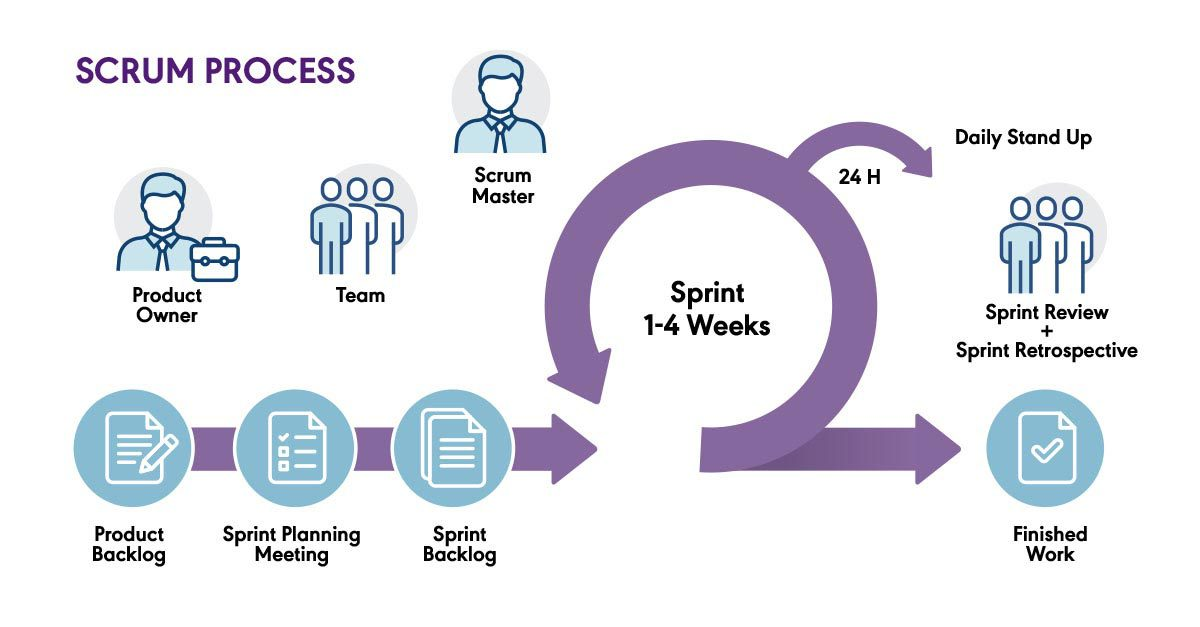
\includegraphics[scale=0.4]{Figures/Scrum.jpg}
    \caption{Processus Scrum}
    \label{fig:scrum}
\end{figure}
\newpage

Les principales étapes du processus Scrum sont les suivantes :

\begin{description}
    \item[\textbf{Product Backlog}] L’ensemble des fonctionnalités, améliorations et corrections à développer est recensé dans le product backlog. Cette liste est priorisée par le Product Owner en fonction des objectifs du projet et des besoins des utilisateurs.
    \item[\textbf{Planification du Sprint}] Au début de chaque sprint, l’équipe sélectionne les éléments du product backlog à réaliser pendant le sprint. Ces éléments constituent le sprint backlog.
    \item[\textbf{Exécution du Sprint}] L’équipe de développement travaille de manière collaborative pour implémenter les fonctionnalités sélectionnées. Des réunions quotidiennes (\textit{daily Scrum}) permettent de suivre l’avancement, de discuter des obstacles et d’ajuster les tâches si nécessaire.
    \item[\textbf{Revue de Sprint}] À la fin du sprint, l’équipe présente le travail accompli aux parties prenantes. Les retours sont recueillis afin d’améliorer le produit et le processus.
    \item[\textbf{Rétrospective du Sprint}] L’équipe analyse ce qui a bien fonctionné, ce qui peut être amélioré, et définit des actions pour optimiser le sprint suivant.
\end{description}

\subsection{Méthodologie pour la partie IA}

Pour la partie intelligence artificielle du projet MindCare-AI, la méthodologie \textbf{CRISP-DM} (Cross-Industry Standard Process for Data Mining) a été adoptée. Cette approche structurée et itérative est particulièrement adaptée aux projets de Data Science et d’IA. Elle a guidé le développement aussi bien du module d’analyse des signes vitaux que du module chatbot. Voici comment les étapes ont été appliquées :

\begin{enumerate}
    \item \textbf{Compréhension du métier} : Définition des objectifs du projet, tels que l’estimation automatisée des signes vitaux (fréquence cardiaque, pression artérielle) à partir d’images faciales, et la mise en place d’un chatbot conversationnel pour l’accompagnement psychologique et la recommandation personnalisée.
    \item \textbf{Compréhension des données} : Analyse des sources de données utilisées pour l’entraînement des modèles (par exemple, la base PPG-DaLiA pour les signes vitaux, corpus de dialogues pour le chatbot), compréhension des variables démographiques et des signaux physiologiques extraits des images, ainsi que des intentions et émotions dans les conversations.
    \item \textbf{Préparation des données} : Prétraitement des images (décodage, détection du visage, extraction des régions d’intérêt), extraction de caractéristiques pertinentes (features temporelles, fréquentielles et démographiques), normalisation et sélection des variables pour l’IA. Pour le chatbot, nettoyage et structuration des données textuelles, annotation des émotions et des intentions.
    \item \textbf{Modélisation} : Entraînement de modèles de classification supervisée (Gradient Boosting pour les signes vitaux, modèles de deep learning pour la détection d’émotions), intégration de modèles de langage (LLM) pour le chatbot, et validation croisée pour optimiser la performance.
    \item \textbf{Évaluation} : Validation des modèles sur des jeux de données tests, mesure de la précision, du rappel et du score F1 pour l’IA, et analyse de la pertinence et de la qualité des réponses pour le chatbot.
    \item \textbf{Déploiement} : Intégration des modèles entraînés dans l’API Flask du projet : le modèle d’analyse des signes vitaux est utilisé en temps réel pour traiter les images envoyées par les utilisateurs, tandis que le chatbot gère les conversations, l’évaluation du stress et la recommandation musicale personnalisée.
\end{enumerate}

La figure suivante illustre les différentes étapes de la méthodologie CRISP-DM appliquées à MindCare-AI.

\begin{figure}[H]
    \centering
    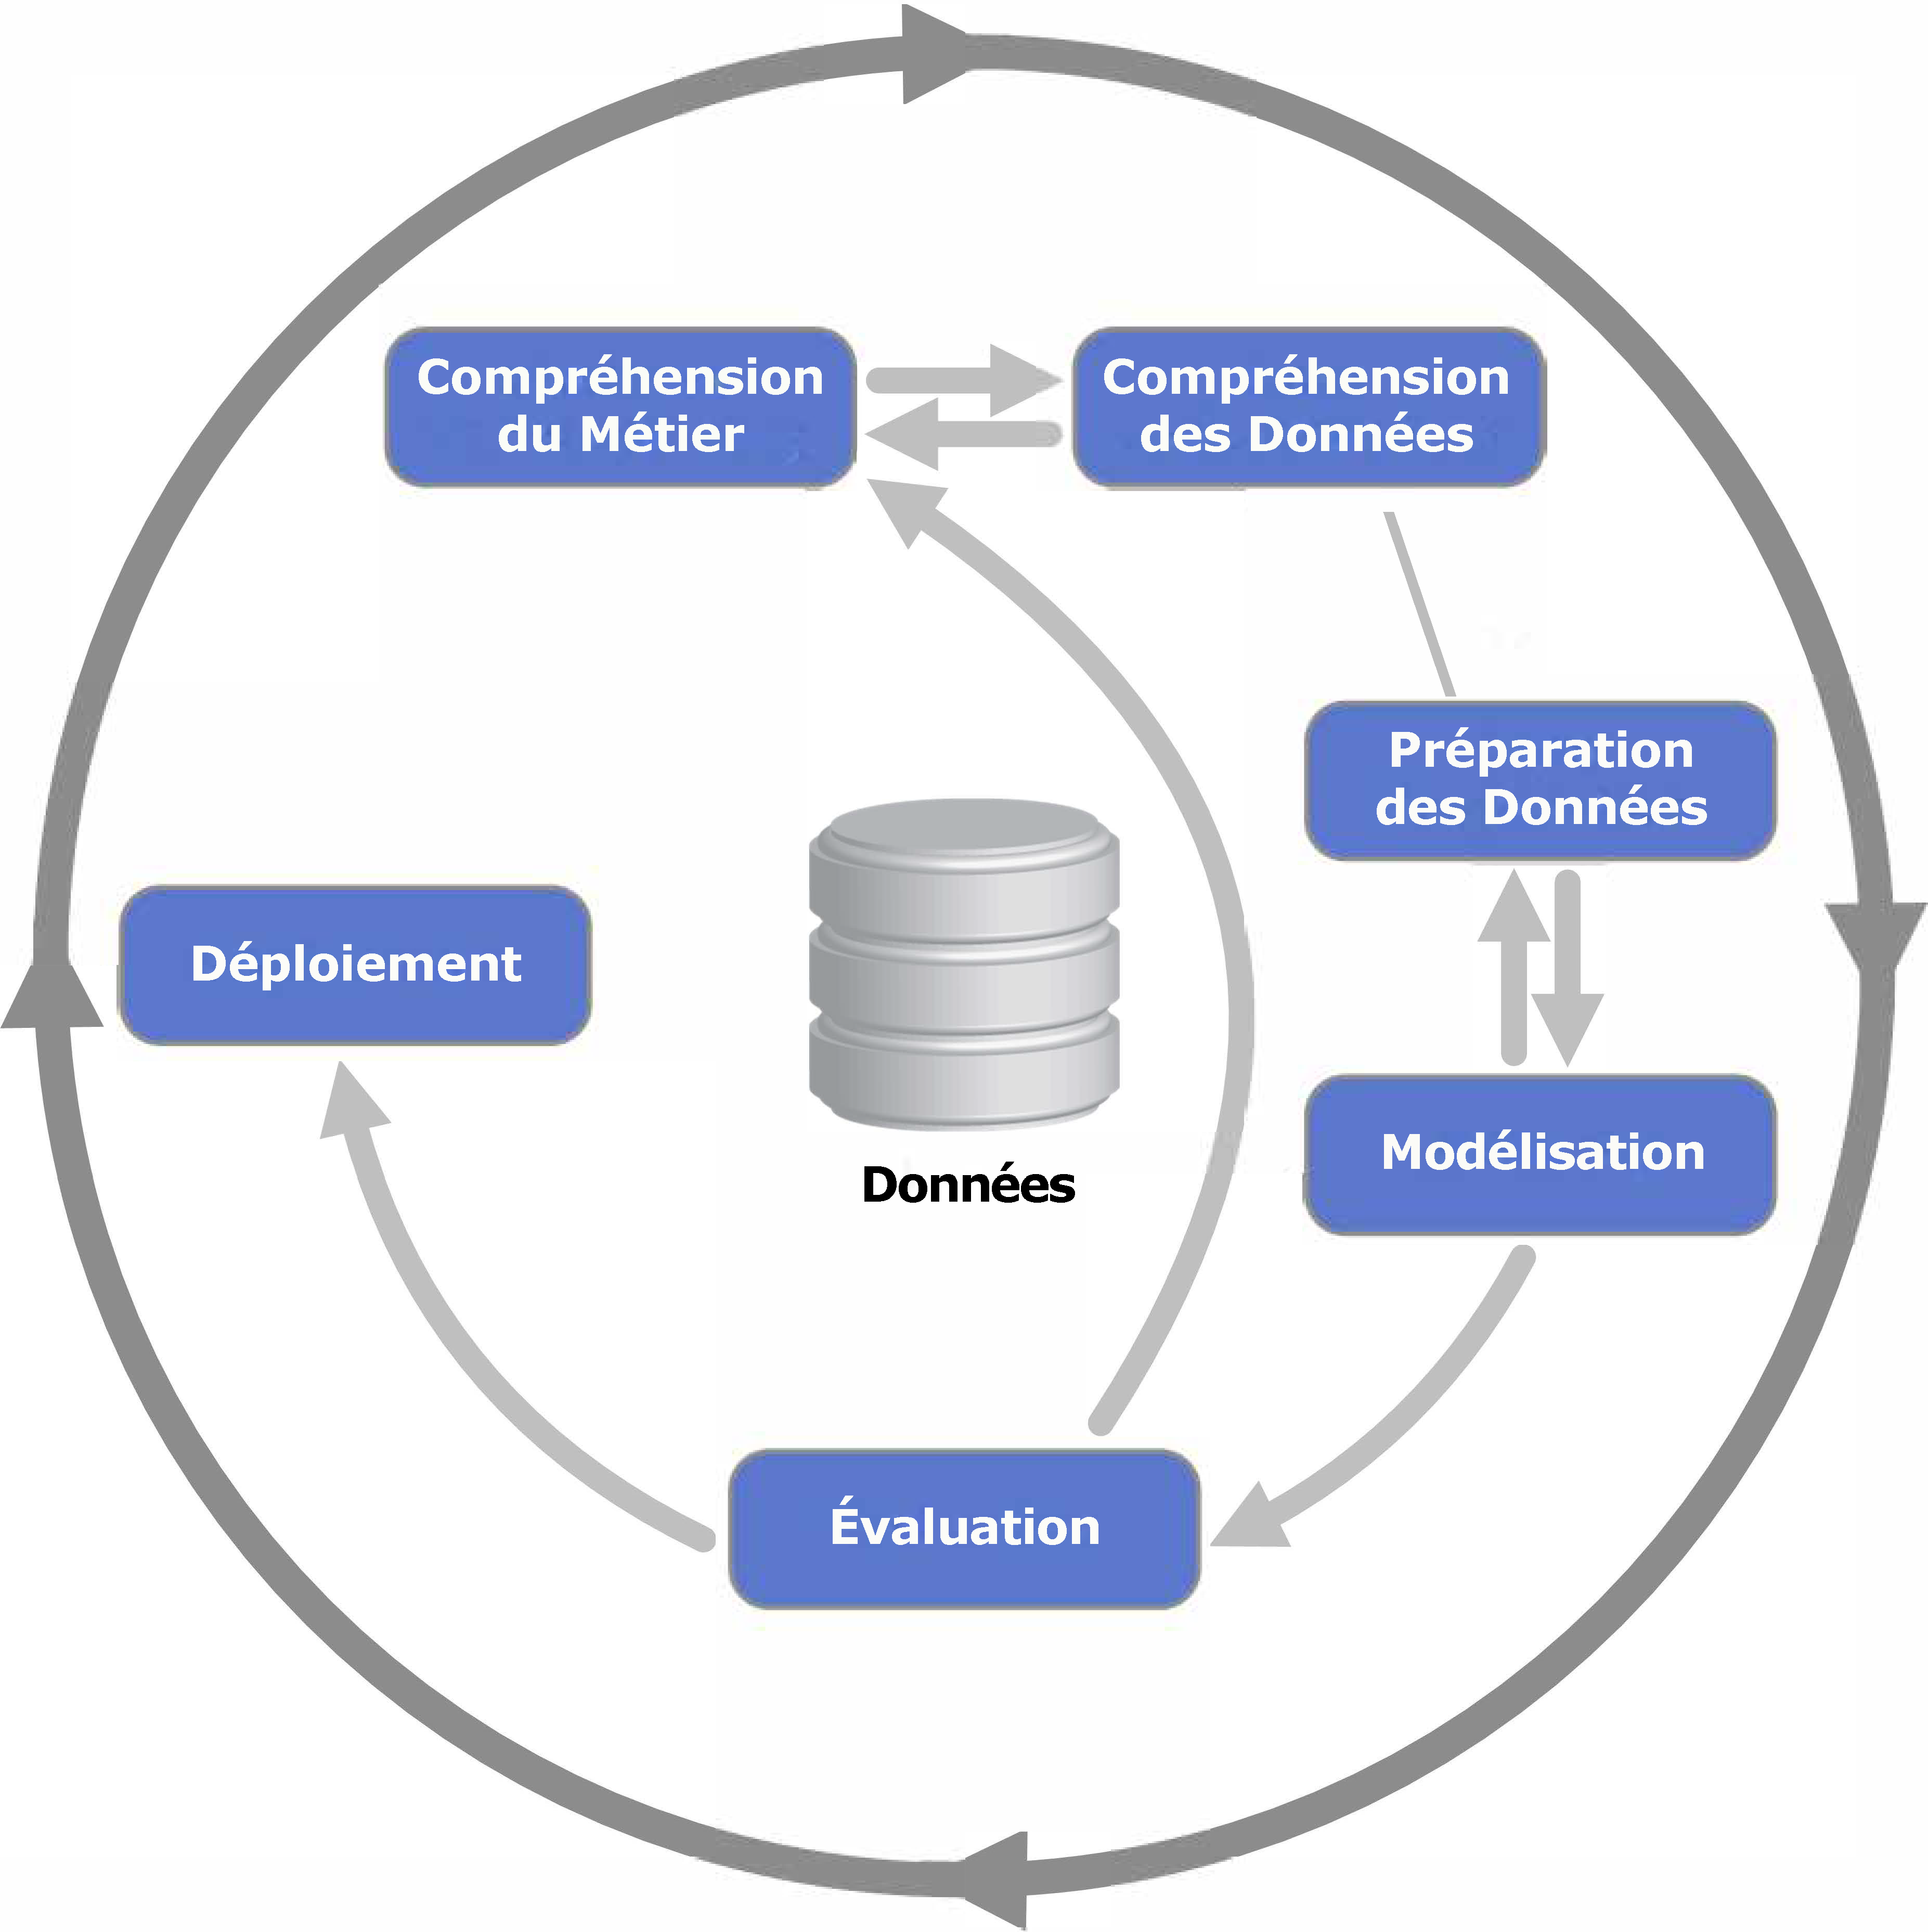
\includegraphics[width=0.8\textwidth]{Figures/Diagramme_du_Processus_CRISP-DM.png}
    \caption{Méthodologie CRISP-DM }
\end{figure}


\section{Conclusion}

En conclusion, ce chapitre a permis d’établir le cadre général du projet MindCare-AI. Nous avons présenté la société d’accueil, exposé le contexte et les enjeux liés à la santé mentale, puis formulé la problématique à laquelle nous avons souhaité répondre. Nous avons également détaillé la solution innovante proposée, en mettant en avant ses différents axes, et expliqué les méthodologies adoptées pour mener à bien le projet. Ces éléments constituent les fondations nécessaires à la compréhension des choix techniques et organisationnels qui seront approfondis dans les chapitres suivants.